\documentclass[10pt,a4paper]{article}
\usepackage[utf8]{inputenc}
\usepackage{amsmath}
\usepackage{amsfonts}
\usepackage{amssymb}
\usepackage{graphicx}
\usepackage[normalem]{ulem}
\useunder{\uline}{\ul}{}
\author{Brock Ellefson}
\title{CSCI338 HW4}
\begin{document}
\maketitle
\section*{Question 1}
Let $\beta$ be the set of all infinite sequences over $\lbrace$a,b$\rbrace$. Show that $\beta$ is uncountable,
using a proof by diagonalization.\\
Assume that $\beta$ is countable, then we can list them as $\beta$$_{1}$ , $\beta$$_{2}$
\begin{table}[h]
\centering
\begin{tabular}{l|lll}
i & {\ul } & f(i) &     \\ \hline
1 & b$_{11}$    & b$_{12}$  & b$_{13}$ \\
2 & b$_{21}$    & b$_{22}$  & b$_{23}$ \\
3 & b$_{31}$    & b$_{32}$  & b$_{33}$
\end{tabular}
\end{table}
\\Now construct an x such that the i$^{th}$ bit of x is $\neq$ the i$^{th}$ bit of $\beta$
\begin{table}[h]
\centering
\begin{tabular}{l|lll}
i & {\ul } & f(i) &   \\ \hline
1 & a      & a & a... \\
2 & b      & a & b... \\
3 & b      & b & b...
\end{tabular}
\end{table}
\\Lets define x as x = (b, b, a...) thus making x $\neq$ $\beta$ for any i$^{th}$ sequence in the i$^{th}$ bit. Therefore $\beta$ is uncountable.

\section*{Question 2}
Let T = $\lbrace$(i,j,k)$\mid$ i,j,k $\epsilon$ N $\rbrace$. Show that T is countable.\\
By definition, the set T is countable iff:\\
If there exists an injective function f from T to the natural numbers\\
If f is surjective\\
If T has a one-to-one correspondence with natural numbers\\
\\\\
Construct a 1-1 and onto function f: T $\rightarrow$ N\\
We know that A = $\lbrace$(i,j)$\mid$ i,j $\epsilon$ N $\rbrace$ is countable\\
The function g((i,j),k) = (i + j)(i + j + 1)/2 + j is a 1-1 correspondence from T on N\\
Assume that f($<$i,j,k$>$) = f($<$i$^{'}$, j$^{'}$, k$^{'}$$>$)\\
Therefore g($<$g($<$i,j$>$,k)$>$) = g($<$g($<$i$^{'}$,j$^{'}$$>$,k$^{'}$)$>$)\\
This makes g a 1-1, therefore f is 1-1\\
\\
Since n $\epsilon$ N, then g($<$m,k$>$) = n for some m,k that is also in N\\
g($<$i,j$>$) = m for some i,j in N\\
Therefore f($<$i,j,k$>$) = g($<$m,k$<$) = g($<$g($<$i,j$>$),k$>$)\\
Therefore T is countable.
\section*{Question 3}
Show that INFINITE$_{PDA}$ is decidable\\
To decide INFINITE$_{PDA}$ convert PDA into equivalent CFG, let P be the pumping length. Construct regular language R that accepts strings longer than P. Intersect of CFL and regular languages is a CFL. Test this intersection for emptiness, accept if L of the intersection is empty, reject otherwise.
\section*{Question 4}
ODD$_{TM}$ = $\lbrace$ $<$M$>$ $\mid$ M is a TM and L(M) contains only strings of odd length $\rbrace$
Prove that ODD$_{TM}$ is undecidable.\\
\\
Reduce ALL$_{TM}$ to ODD$_{TM}$\\
Assume that ODD$_{TM}$ is decidable. Let R be a decider for ODD$_{TM}$ and have R decide T on w:\\
if R accepts, accept\\
if R rejects, reject\\
\\
O(T) us a decuder for ODD$_{TM}$. Now build a decider for A$_{TM}$. This is impossible, therefore ODD$_{TM}$ is undecideable
\section*{Question 5}
Show that EQ$_{CFG}$ is undecidable.\\
(This can also be proven via rice's theorem)
Assume that EQ$_{CFG}$ is decideable\\
EQ$_{CFG}$ = $\lbrace$ $<$G,H$>$ $\mid$ G,H are CFG's and L(G) = L(H) $\rbrace$
\\
Reduce ALL$_{CFG}$ to EQ$_{CFG}$ Such That:
\\
ALL$_{CFG}$ = $\lbrace$ $<$G$>$ $\mid$ G is a CFG's and L(G) = $\Sigma$$^{\ast}$ $\rbrace$
\\
Let R be a decider for EQ$_{CFG}$ and construct TM S to decide ALL$_{CFG}$.
\\
Construct CFG T such that L(T) = $\Sigma$$^{\ast}$
\begin{enumerate}
  \item Run R on input $<$G,T$_{0}$$>$
  \item If R accepts, accept.
  \item If R rejects, reject 
\end{enumerate}
R decides if L(G) = L(T). S decides ALL$_{CFG}$ but it is undecidable, therefore EQ$_{CFG}$ must also be undecidable 

\section*{Question 6}
Show that EQ$_{CFG}$ is co-Turing-recognizable.\\\\
A language is co-turning recognizable if and only if its complement is a turning-recognizable language.\\
\\
Convert G and H into Chomsky normal form. Begin iterating through the strings in $\Sigma$$^{\ast}$. If both G or H can generate or not generate the string a TM will continue on the interation of strings, however, if one CFG accepts a string and the other does not, that means that the CFG's are not equvilent and the TM accepts. Therefore EQ$_{CFG}$  is co-turning recognizeable.
\section*{Question 7}
Post Correspondence Problem.\\
	\begin{figure}[h]
		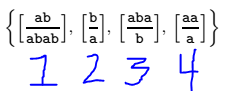
\includegraphics[scale = .5]{338q7.png}
  		\label{fig:PCP}
	\end{figure}
\\
A working string is:\\
11132124234244\\
ababababababbaababaaabaaa
\end{document}
